% Source: graduate-coursework/Research/Intro_to_Agents/handouts/Part6_MultiTier_Architecture.tex

\documentclass[border=4pt]{standalone}
\usepackage{amsmath,amssymb,amsfonts}
\usepackage[T1]{fontenc}
\usepackage{graphicx}
\usepackage{lmodern}
\usepackage{tikz}
\usepackage{xcolor}
\usetikzlibrary{shapes,arrows.meta,positioning,calc,fit,backgrounds,chains,decorations.pathreplacing}

\definecolor{UofSCGarnet}{HTML}{73000a}
\definecolor{UofSCBlack}{HTML}{000000}
\definecolor{UofSCWhite}{HTML}{ffffff}
\definecolor{UofSCRose}{HTML}{CC2E40}
\definecolor{UofSCAtlantic}{HTML}{466A9F}
\definecolor{UofSCCongaree}{HTML}{1F414D}
\definecolor{UofSCHorseshoe}{HTML}{65780B}
\definecolor{UofSCGrass}{HTML}{CED318}
\definecolor{UofSCHoneycomb}{HTML}{A49137}
\definecolor{UofSC90Black}{HTML}{363636}
\definecolor{UofSC70Black}{HTML}{5C5C5C}
\definecolor{UofSC50Black}{HTML}{A2A2A2}
\definecolor{UofSCWarmGrey}{HTML}{676156}
\definecolor{UofSCSandstorm}{HTML}{FFF2E3}
\definecolor{UofSCDarkGarnet}{HTML}{570008}
\definecolor{UofSCAzalea}{HTML}{844247}

\tikzset{
    % Base node style
    basenode/.style={
        draw=UofSCBlack,
        fill=UofSCWhite,
        line width=0.8pt,
        minimum height=0.8cm,
        minimum width=2cm,
        align=center,
        font=\small
    },
    % Strategy layer style
    strategynode/.style={
        basenode,
        fill=UofSCGarnet,
        text=UofSCWhite,
        minimum height=1cm,
        minimum width=4cm
    },
    % Planning layer style
    planningnode/.style={
        basenode,
        fill=UofSCAtlantic,
        text=UofSCWhite,
        minimum height=0.9cm,
        minimum width=3.5cm
    },
    % Execution layer style
    execnode/.style={
        basenode,
        fill=UofSCCongaree,
        text=UofSCWhite,
        minimum height=0.8cm,
        minimum width=2.5cm
    },
    % Generic box
    genericbox/.style={
        basenode,
        minimum width=2.8cm
    },
    % Arrow styles (straight lines only)
    myarrow/.style={
        ->,
        >=Stealth,
        line width=0.8pt,
        draw=UofSCBlack
    },
    % Bidirectional arrow
    biarrow/.style={
        <->,
        >=Stealth,
        line width=0.8pt,
        draw=UofSCBlack
    },
    % Phase box style
    phasebox/.style={
        basenode,
        minimum width=3.5cm,
        minimum height=1.2cm,
        font=\small\bfseries
    },
    % Small box
    smallbox/.style={
        basenode,
        minimum width=1.5cm,
        minimum height=0.6cm,
        font=\scriptsize
    },
    % Leader node
    leadernode/.style={
        basenode,
        fill=UofSCGarnet,
        text=UofSCWhite,
        minimum width=3cm,
        minimum height=1cm
    },
    % Worker node
    workernode/.style={
        basenode,
        fill=UofSC70Black,
        text=UofSCWhite,
        minimum width=1.2cm,
        minimum height=0.7cm,
        font=\scriptsize
    }
}

\begin{document}
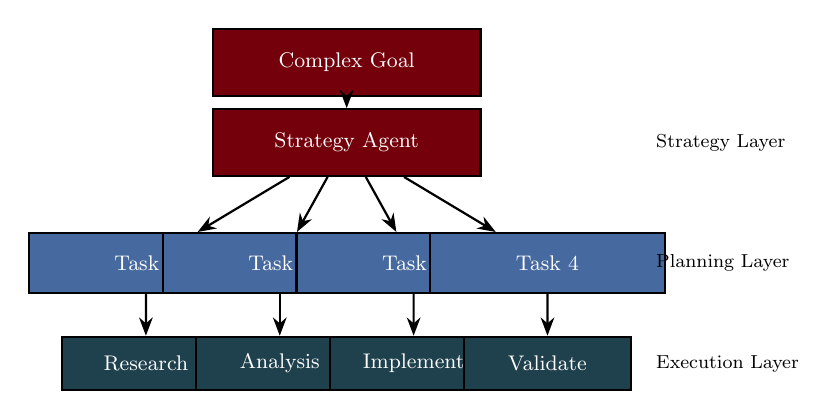
\begin{tikzpicture}[scale=0.85, transform shape]
        % Top level
        \node[strategynode] (goal) at (0,5) {Complex Goal};
        \node[strategynode] (strategy) at (0,3.8) {Strategy Agent};

        % Planning level
        \node[planningnode] (p1) at (-3,2) {Task 1};
        \node[planningnode] (p2) at (-1,2) {Task 2};
        \node[planningnode] (p3) at (1,2) {Task 3};
        \node[planningnode] (p4) at (3,2) {Task 4};

        % Execution level
        \node[execnode] (e1) at (-3,0.5) {Research};
        \node[execnode] (e2) at (-1,0.5) {Analysis};
        \node[execnode] (e3) at (1,0.5) {Implement};
        \node[execnode] (e4) at (3,0.5) {Validate};

        % Arrows
        \draw[myarrow] (goal) -- (strategy);
        \draw[myarrow] (strategy) -- (p1);
        \draw[myarrow] (strategy) -- (p2);
        \draw[myarrow] (strategy) -- (p3);
        \draw[myarrow] (strategy) -- (p4);

        \draw[myarrow] (p1) -- (e1);
        \draw[myarrow] (p2) -- (e2);
        \draw[myarrow] (p3) -- (e3);
        \draw[myarrow] (p4) -- (e4);

        % Labels
        \node[font=\footnotesize,right] at (4.5,3.8) {Strategy Layer};
        \node[font=\footnotesize,right] at (4.5,2) {Planning Layer};
        \node[font=\footnotesize,right] at (4.5,0.5) {Execution Layer};
    \end{tikzpicture}
\end{document}
